

\tikzset{every picture/.style={line width=0.75pt}} %set default line width to 0.75pt        

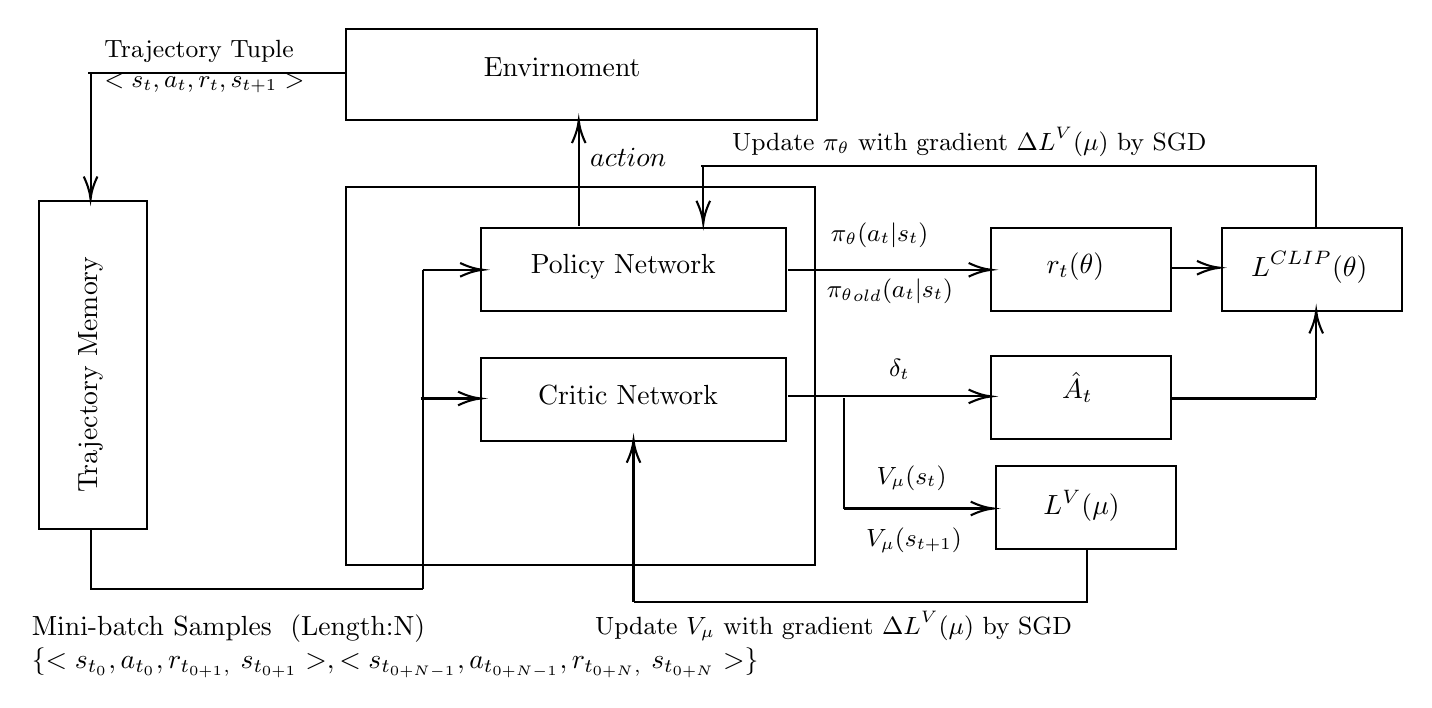
\begin{tikzpicture}[x=0.75pt,y=0.75pt,yscale=-1,xscale=1]
%uncomment if require: \path (0,338); %set diagram left start at 0, and has height of 338

%Shape: Rectangle [id:dp9978943115484824] 
\draw   (26.8,246.3) -- (26.8,88.3) -- (78.8,88.3) -- (78.8,246.3) -- cycle ;

%Shape: Rectangle [id:dp05267034608632715] 
\draw   (174.8,5.14) -- (401.8,5.14) -- (401.8,49.3) -- (174.8,49.3) -- cycle ;
%Shape: Rectangle [id:dp04578612721398789] 
\draw   (174.8,81.3) -- (400.8,81.3) -- (400.8,263.3) -- (174.8,263.3) -- cycle ;
%Shape: Rectangle [id:dp479111495997272] 
\draw   (240,101) -- (386.8,101) -- (386.8,141) -- (240,141) -- cycle ;

%Shape: Rectangle [id:dp3592684590066768] 
\draw   (240,164) -- (386.8,164) -- (386.8,204) -- (240,204) -- cycle ;

%Shape: Rectangle [id:dp5726876145364976] 
\draw   (485.5,101) -- (572.3,101) -- (572.3,141) -- (485.5,141) -- cycle ;

%Shape: Rectangle [id:dp8126568031433179] 
\draw   (597,101) -- (683.8,101) -- (683.8,141) -- (597,141) -- cycle ;

%Shape: Rectangle [id:dp24057721244799102] 
\draw   (488,216) -- (574.8,216) -- (574.8,256) -- (488,256) -- cycle ;

%Shape: Rectangle [id:dp21651348351379074] 
\draw   (485.5,163) -- (572.3,163) -- (572.3,203) -- (485.5,203) -- cycle ;

%Straight Lines [id:da2065459425933598] 
\draw    (313.4,281.3) -- (313.4,205.3) ;
\draw [shift={(313.4,203.3)}, rotate = 450] [color={rgb, 255:red, 0; green, 0; blue, 0 }  ][line width=0.75]    (10.93,-3.29) .. controls (6.95,-1.4) and (3.31,-0.3) .. (0,0) .. controls (3.31,0.3) and (6.95,1.4) .. (10.93,3.29)   ;
%Straight Lines [id:da5843246843678724] 
\draw    (387.8,182.3) -- (483.8,182.3) ;
\draw [shift={(485.8,182.3)}, rotate = 180] [color={rgb, 255:red, 0; green, 0; blue, 0 }  ][line width=0.75]    (10.93,-3.29) .. controls (6.95,-1.4) and (3.31,-0.3) .. (0,0) .. controls (3.31,0.3) and (6.95,1.4) .. (10.93,3.29)   ;
%Straight Lines [id:da5820279370707651] 
\draw    (387.8,121.3) -- (483.8,121.3) ;
\draw [shift={(485.8,121.3)}, rotate = 180] [color={rgb, 255:red, 0; green, 0; blue, 0 }  ][line width=0.75]    (10.93,-3.29) .. controls (6.95,-1.4) and (3.31,-0.3) .. (0,0) .. controls (3.31,0.3) and (6.95,1.4) .. (10.93,3.29)   ;
%Straight Lines [id:da03477812258414015] 
\draw    (414.8,236.3) -- (484.8,236.3) ;
\draw [shift={(486.8,236.3)}, rotate = 180] [color={rgb, 255:red, 0; green, 0; blue, 0 }  ][line width=0.75]    (10.93,-3.29) .. controls (6.95,-1.4) and (3.31,-0.3) .. (0,0) .. controls (3.31,0.3) and (6.95,1.4) .. (10.93,3.29)   ;
%Straight Lines [id:da09026891505962009] 
\draw    (414.8,183.3) -- (414.8,236.3) ;
%Shape: Right Angle [id:dp09688091613107686] 
\draw   (531.8,256) -- (531.8,281.3) -- (313.4,281.3) ;
%Straight Lines [id:da10002566422487891] 
\draw    (51.8,26.3) -- (51.8,85.3) ;
\draw [shift={(51.8,87.3)}, rotate = 270] [color={rgb, 255:red, 0; green, 0; blue, 0 }  ][line width=0.75]    (10.93,-3.29) .. controls (6.95,-1.4) and (3.31,-0.3) .. (0,0) .. controls (3.31,0.3) and (6.95,1.4) .. (10.93,3.29)   ;
%Straight Lines [id:da14348663665795947] 
\draw    (210.8,183.3) -- (237.8,183.3) ;
\draw [shift={(239.8,183.3)}, rotate = 180] [color={rgb, 255:red, 0; green, 0; blue, 0 }  ][line width=0.75]    (10.93,-3.29) .. controls (6.95,-1.4) and (3.31,-0.3) .. (0,0) .. controls (3.31,0.3) and (6.95,1.4) .. (10.93,3.29)   ;
%Straight Lines [id:da1581117014190938] 
\draw    (211.8,121.3) -- (238.8,121.3) ;
\draw [shift={(240.8,121.3)}, rotate = 180] [color={rgb, 255:red, 0; green, 0; blue, 0 }  ][line width=0.75]    (10.93,-3.29) .. controls (6.95,-1.4) and (3.31,-0.3) .. (0,0) .. controls (3.31,0.3) and (6.95,1.4) .. (10.93,3.29)   ;
%Straight Lines [id:da3327122153372011] 
\draw    (211.8,121.3) -- (211.8,275.3) ;
%Shape: Right Angle [id:dp7457457500271234] 
\draw   (211.8,275.3) -- (51.8,275.3) -- (51.8,246) ;
%Straight Lines [id:da24558256059318717] 
\draw    (174.8,26.3) -- (50.8,26.3) ;
%Straight Lines [id:da1907077659365608] 
\draw    (287,100) -- (287,51.3) ;
\draw [shift={(287,49.3)}, rotate = 450] [color={rgb, 255:red, 0; green, 0; blue, 0 }  ][line width=0.75]    (10.93,-3.29) .. controls (6.95,-1.4) and (3.31,-0.3) .. (0,0) .. controls (3.31,0.3) and (6.95,1.4) .. (10.93,3.29)   ;
%Straight Lines [id:da25181356746653694] 
\draw    (347,71.3) -- (347,97) ;
\draw [shift={(347,99)}, rotate = 270] [color={rgb, 255:red, 0; green, 0; blue, 0 }  ][line width=0.75]    (10.93,-3.29) .. controls (6.95,-1.4) and (3.31,-0.3) .. (0,0) .. controls (3.31,0.3) and (6.95,1.4) .. (10.93,3.29)   ;
%Shape: Right Angle [id:dp9296457308111634] 
\draw   (345.8,71.3) -- (642.3,71.3) -- (642.3,101) ;
%Straight Lines [id:da7729636916978786] 
\draw    (642.3,183.3) -- (642.3,143) ;
\draw [shift={(642.3,141)}, rotate = 450] [color={rgb, 255:red, 0; green, 0; blue, 0 }  ][line width=0.75]    (10.93,-3.29) .. controls (6.95,-1.4) and (3.31,-0.3) .. (0,0) .. controls (3.31,0.3) and (6.95,1.4) .. (10.93,3.29)   ;
%Straight Lines [id:da8163897958062174] 
\draw    (572.8,183.3) -- (642.3,183.3) ;
%Straight Lines [id:da9600198123912971] 
\draw    (572.8,120.3) -- (593.8,120.3) ;
\draw [shift={(595.8,120.3)}, rotate = 180] [color={rgb, 255:red, 0; green, 0; blue, 0 }  ][line width=0.75]    (10.93,-3.29) .. controls (6.95,-1.4) and (3.31,-0.3) .. (0,0) .. controls (3.31,0.3) and (6.95,1.4) .. (10.93,3.29)   ;


% Text Node
\draw (44.3,230.3) node [anchor=north west][inner sep=0.75pt]  [rotate=-270] [align=left] {Trajectory Memory};
% Text Node
\draw (509.4,226) node [anchor=north west][inner sep=0.75pt]   [align=left] {$\displaystyle L^{V}( \mu )$};
% Text Node
\draw (518.4,169) node [anchor=north west][inner sep=0.75pt]   [align=left] {$\displaystyle \hat{A}_{t}$};
% Text Node
\draw (510.9,111.5) node [anchor=north west][inner sep=0.75pt]   [align=left] {$\displaystyle r_{t}( \theta )$};
% Text Node
\draw (609.4,111) node [anchor=north west][inner sep=0.75pt]   [align=left] {$\displaystyle L^{CLIP}( \theta )$};
% Text Node
\draw (265.9,175.5) node [anchor=north west][inner sep=0.75pt]   [align=left] {Critic Network};
% Text Node
\draw (262.4,112.5) node [anchor=north west][inner sep=0.75pt]   [align=left] {Policy Network};
% Text Node
\draw (239.8,17.65) node [anchor=north west][inner sep=0.75pt]   [align=left] {Envirnoment};
% Text Node
\draw (407,97) node [anchor=north west][inner sep=0.75pt]  [font=\small] [align=left] {$\displaystyle \pi _{\theta }( a_{t} |s_{t})$};
% Text Node
\draw (405,124) node [anchor=north west][inner sep=0.75pt]  [font=\small] [align=left] {$\displaystyle {\pi _{\theta }}_{old}( a_{t} |s_{t})$};
% Text Node
\draw (435,163) node [anchor=north west][inner sep=0.75pt]  [font=\small] [align=left] {$\displaystyle \delta _{t}$};
% Text Node
\draw (429,214) node [anchor=north west][inner sep=0.75pt]  [font=\small] [align=left] {$\displaystyle V_{\mu }( s_{t})$};
% Text Node
\draw (424,244) node [anchor=north west][inner sep=0.75pt]  [font=\small] [align=left] {$\displaystyle V_{\mu }( s_{t+1})$};
% Text Node
\draw (57,9) node [anchor=north west][inner sep=0.75pt]  [font=\small] [align=left] {Trajectory Tuple\\$\displaystyle < s_{t} ,a_{t} ,r_{t} ,s_{t+1}  >$};
% Text Node
\draw (22,286) node [anchor=north west][inner sep=0.75pt]   [align=left] {Mini-batch Samples \ (Length:N)\\$\displaystyle \{< s_{t_{0}} ,a_{t_{0}} ,r_{t_{0+1} ,\ } s_{t_{0+1}}  >,\dotsc < s_{t_{0+N-1}} ,a_{t_{0+N-1}} ,r_{t_{0+N} ,\ } s_{t_{0+N}}  >\}$};
% Text Node
\draw (293.4,284.3) node [anchor=north west][inner sep=0.75pt]  [font=\small] [align=left] {Update $\displaystyle V_{\mu }$ with gradient $\displaystyle \Delta L^{V}( \mu )$ by SGD};
% Text Node
\draw (359.4,51) node [anchor=north west][inner sep=0.75pt]  [font=\small] [align=left] {Update $\displaystyle \pi _{\theta }$ with gradient $\displaystyle \Delta L^{V}( \mu )$ by SGD};
% Text Node
\draw (291,61.3) node [anchor=north west][inner sep=0.75pt]   [align=left] {$\displaystyle action$};


\end{tikzpicture}